\section{Reactive Process}
\label{sec:process}

As discussed earlier, the design of \hpl{} should improve the flexibility to introduce 
support for managing variabilities on new SPL assets, and thus evolve the configurability 
space of \hpl{}. In this section we describe a process (Figure~\ref{fig:process} shows the corresponding BPMN diagram) that could guide domain engineers to proceed in this task. 
It is important to note that we have designed this process based on our experience for 
evolving the versions of \hpl{} to support several assets (use cases, business processes, requirements and code). Therefore, it focuses on the reactive process to introduce new asssets into \hpl. 

Three roles contribute to this process, which are represented as the lanes in Figure~\ref{fig:process}. Customers start the reactive 
process in \hpl{} demanding a Hephaestus tool with new requirements. Application engineers consider the new requirements,
specify and map the requirements for the features of \hpl{}, and evaluate whether the requirements are 
already supported by \hpl. If so, they generate the \hpl{} product with the desired configuration, 
testing and delivering it to the customer. If \hpl{} does not support the customer tool's requirements yet, the application 
engineers submit to the domain engineer the demand for evolving \hpl{} to support the new requirements (assets).

The domain engineers here comprise two distinct roles: \emph{asset domain expert} that defines and 
implements the artifacts of the new assets; and \emph{domain engineer of \hpl{}} that evaluates the impact and integrates the artifacts 
of the new asset into \hpl. The \emph{asset domain expert} executes activities concerning the new artifact, by providing its implementation in terms of data types, transformations, parsers, and output format functions. It corresponds the 
\textit{Define asset type structures}, \textit{Define asset transformations}, \textit{Implement asset parser} and \textit{Implement asset output format} activities in Figure~\ref{fig:process}.
No order is specified among these tasks because they are normally 
carried out iteratively. The \textit{domain engineer of \hpl{}} assesses whether the introduction of a new asset needs to update the \hpl{} 
Kernel's APIs (high and low level transformations); integrates the new asset's artifacts into \hpl{} infrastruture; updates the metadata strutures inserting references to the new 
asset; updates Hephaestus-PL's FM and CK using the guidance of safe evolution templates of software product 
lines defined~\cite{gpce11}; and validates the new asset by generating a new \hpl{} product with the selected new asset and checking 
the correctness of the generated source code. If the generated product is a valid Hephaestus product 
then the domain engineer's activities are finalized.

%This lane involves activities concerning the new artifact, i.e., providing its implementation in terms of data types, their transformations, parsers, and output format functions. No order is specified since these are normally carried out in a iterative fashion. 
%The first activity of the field engineer to evaluate the impact of HPL to support the new asset.

%In addition to these activities, this lane involves other activities to integrate the new asset to the \hp{} product line, how to introduce new modules implemented to new artifact into \hpl's infrastructure, update Hephaestus-PL's FM and CK using the guidance of safe evolution templates of software product lines defined in ~\cite{gpce11} and update the asset meta data structures that support the metaprogramming operations to manage the variability of \hpl.
%Finally, it is necessary to execute the derivation of a simplified \hpl{} product with only the new asset to validate the evolution of \hpl{}. If the generated product is a valid Hephaestus product then the domain engineer's activities are finalized. The validation of Hephaestus product can be done using a checklist. Otherwise, if the generated product is not valid or does not meet the specification of the new asset, additional activities are conducted by the domain engineer to assess possible needs for changes in the metaprogramming operations, in the asset meta data structures or in the contents of the meta data structures of the new asset until deriving a valid product.


%The lane corresponding to the domain engineer involves activities concerning the new artifact, i.e., providing its implementation in terms of data types, their transformations,  parsers, and output format functions. No order is specified since these are normally carried out in a iterative fashion. The lane corresponding to the application engineer involve integrating new modules implemented to new artifact into \hpl's infrastructure, and correspondingly updating its feature model, configuration knowledge, and asset meta data structures.
%Then,  it is necessary to execute the derivation a product with the new asset to validate the evolution of Hephaestus-PL. If the result is a valid Hephaestus product then the reactive process is finalized. The validation of Hephaestus product can be done using a checklist. Otherwise, the domain engineer analyses the errors or improper behavior of generated product Hephaestus instance and execute a set of activities to correct the error with possible needs for changes in the operations of metaprogramming and in the asset meta data structures. After that, we execute the test of the generation of an Hephaestus instance with the new asset again and we need to execute a regression test to validate that changes made in metaprogramming and in the asset meta data structures did not impact the generation of products with the assets already owned the Hephaestus-PL.

\subsection{Evolution of Hephaestus-PL to support the Requirement Model asset} \label{sec:evolHplReq}

To illustrate the execution of the reactive process we apresent the evolution of Hephaestus-PL's to support the management of variabilities in the \textit{Requirement Model} asset. The current version of \hpl{} supports \textit{Use Case Model} and \textit{Business Process Model} assets. Figure~\ref{fig:evol-hpl-req} summarizes this scenario of evolution of \hpl{} which we describe below.


\begin{figure*}[bth]
\begin{center}
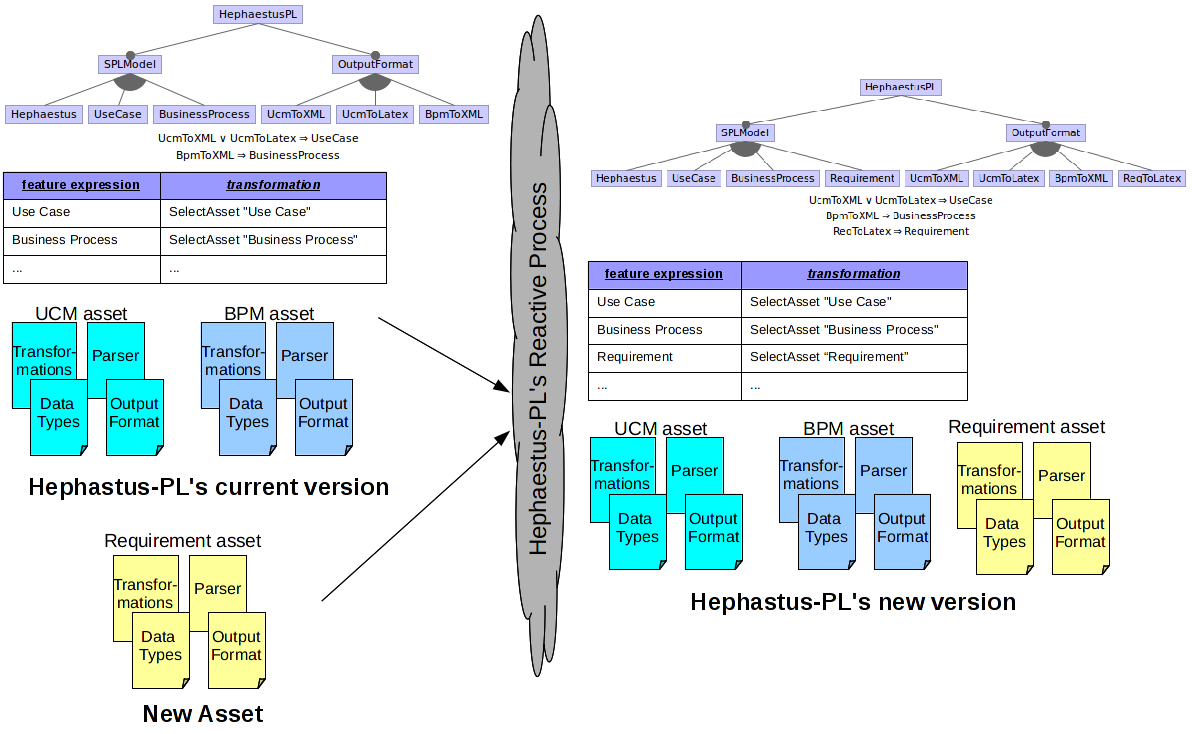
\includegraphics[scale=0.5]{imagens/evol-hpl-req.png}
\end{center}
\caption{Hephaestus-PL's Evolution to introduce the \textit{Requirement} asset.}
\label{fig:evol-hpl-req}
\end{figure*}

%The first release of \hpl{} only supports \textit{use case (UCM)} asset. 
%But, the customer requests a new \hp{} tool that supports BPM product lines. In this case, the customer defining the tool's requirements, i.e., \textit{deriving products of BPM product lines}. 
%Given the need to introduce supporting for Requirement, new requirements for the product line were provided. Because this version of \hpl{} did not support these requirements, there is a need to evolve it to support the management of variabilities in a new asset (BPM).

%The application engineer tries to map this requirement to a feature of Hephaestus-PL's FM and evaluates that \hpl{} has not supported this requirement yet. Then the application engineer submits to the domain engineer a demand for evolution of \hpl{} supporting the new requirement (BPM asset). At first in this level, 

The reactive process to introduce new assets into \hpl{} begins with the \textit{domain engineer} assessing the impacts in Kernel's APIs of \hpl{} to support the \textit{Requirement} asset. It's necessary to analyze whether the high level APIs \--- corresponding to Hephaestus-PL's transformations (\textit{SelectAsset} and \textit{SelectExport}) \--- and low level APIs \--- corresponding to the metaprogramming operations \--- support the specification of new \textit{Requirement} asset. This reactive process considers that the transformations of \hpl{} (\textit{SelectAsset} and \textit{SelectExport}) support new assets, i.e., 
%usually there will be no impact on high-level APIs in \hpl. 
based on our experience, introducing support for variation in a new asset in \hpl{} does not impact the high level APIs. 
%However, the low level APIs may require some adjustments to satisfy the new asset but it represents lower impact. In this case, both the Kernel's APIs support the \textit{Requirement} asset. 

Then, the \textit{asset domain expert} has to implement the four artifacts of \textit{Requirement} asset to evolve \hpl{} supporting this asset. The items below describe what is necessary to define about the new \textit{Requirement} asset:

\textit{(i)} to define the \texttt{RequirementModel} data type and other auxiliary types that represent a set of requirements with their variabilities. The \\ \texttt{RequirementModel} data type is composed by id, name, and description fields (see code snippet in Figure~\ref{fig:code-req-data-type}) and is located in a specific module, i.e., \texttt{ HplAssets.ReqModel.Types.hs} module; 

\begin{figure}
%\begin{code}
\begin{lstlisting}
data Requirement = Requirement {
      reqId :: Id, 
      reqName :: String,
      reqDescription :: String
} deriving (Show, Data, Typeable)        
             
data RequirementModel = RM {
      reqs :: [Requirement]
} deriving (Show, Eq, Data, Typeable)
\end{lstlisting}  
\caption{Definition of \texttt{RequirementModel} data type}
\label{fig:code-req-data-type}
%\end{code}
\end{figure}   


\textit{(ii)} to define the transformations and empty instance function of \textit{Requirement} asset. The transformations specified that managing variabilities in Requirements are \texttt{SelectAllRequirements}, \texttt{SelectRequirements} and \texttt{RemoveRequirements}. The \texttt{emptyReq} is the function which defines a Requirement asset empty instance. It is also necessary to define a data type and a function to comprise all the transformations of Requirement asset to introduce them in a product \hpl{} instance. For example, we defined the \texttt{RequirementTransformation} data type and the \texttt{transformReq} function, respectively. The definition \texttt{RequirementTransformation} must have the clause \texttt{deriving (Show, Eq, Ord)} to allow the ordering and viewing of the Requirement asset's transformations. All definitions of data types to \textit{Requirement} asset must be in \texttt{HplAssets.ReqModel.Types.hs} module. The \texttt{transformReq} function must to have a similar signature of the \texttt{transform} function into \texttt{BaseProduct.hs} module that is a \hpl{} base instance. Besides, a \texttt{transformReq} function must be defined by pattern matching for each constructor declared in the \texttt{RequirementTransformation} data type (see code snippet in Figure~\ref{fig:code-req-transf}).
Both the \texttt{emptyReq} and \texttt{transformReq} functions are implemented in a specific module, i.e., 
\texttt{ HplAssets.Requirements.hs} module. 
These functions must be visible by the \hpl{} kernel to be able to generate a new \hpl{} instance with selected \textit{Requirement} asset; 

\begin{figure}
%\begin{code}
\begin{lstlisting}
data RequirementTransformation = SelectAllRequirements 
                               | SelectRequirements [Id]
                               | RemoveRequirements [Id]
                               deriving (Show, Eq, Ord)
			       
emptyReq :: RequirementModel -> RequirementModel
emptyReq reqmodel = reqmodel { reqs = [] }

transformReq :: RequirementTransformation 
             -> SPLModel 
             -> InstanceModel 
             -> InstanceModel
             
transformReq (SelectAllRequirements) spl product =...
transformReq (SelectRequirements ids) spl product =...
transformReq (RemoveRequirements ids) spl product =...
\end{lstlisting}  
\caption{Definition of \texttt{RequirementModel's} transformations and \texttt{emptyReq} function}
\label{fig:code-req-transf}
%\end{code}
\end{figure}   
 

\textit{(iii)} to implement a new \textit{Requirement} asset parser function to reading the artifacts of Requirement product line from a public representation format such as XML into \texttt{RequirementModel} data type in \hpl.

\textit{(iv)} to implement a new \textit{Requirement} asset output format function, i.e., \texttt{exportReqToLatex} function that enables the exportation of Requirement product instance in the Latex output format out Hephaestus's tool.

After setting the four artifacts of \textit{Requirement} asset, the domain engineer performs the integration of the modules of the new \textit{Requirement} asset into \hpl. She creates a new directory to the \textit{Requirement} asset below the \texttt{HplAssets} directory, i.e., \texttt{ReqModel} directory, and inserts the new asset's modules there, except the \texttt{ HplAssets.Requirements.hs} module with the definitions of \texttt{emptyReq} and \texttt{transformReq} functions which is placed at the same level of \texttt{ReqModel} directory (below the \texttt{HplAssets} directory).

Then, the domain engineer picks up the information of the \textit{Requirement} asset modules and setting the data sets that supporting the execution of low-level APIs of \hpl{} Kernel. This represents to extend the \texttt{AssetMetaData} and \texttt{ExportMetaData} metadata structures defined in \texttt{HplAssets.Hephaestus.MetaData.hs} module to support the new \textit{Requirement} asset. 
Some informations defined in the modules of \textit{Requirement} asset, such as identifiers of data types, fields, functions and modules are inserted in the metadata structures. These informations will be used by metaprogramming support to extend the open data types and open functions in the Hephaestus-PL's base product and generating an instance of \hpl{} with the selected \textit{Requirement} asset. For example, informations about \textit{Requirement} asset such as the data field name and data type to extend the \textit{SPLModel} and \textit{InstanceModel} data types, i.e., \texttt{("splReq","RequirementModel")} and \texttt{("req","RequirementModel")} respectively; the function name that defines a \textit{Requirement} asset empty instance, i.e., \texttt{emptyReq}; the function name that implements the parser of \textit{Requirement} asset, i.e., \texttt{parseRequirementModel}; the name of data type that defines all the Requirement asset transformations, i.e., \texttt{RequirementTransformation}.

After that, the domain engineer updates the Hephaestus-PL's FM and CK defined into \texttt{HplAssets.Hephaestus.MetaData.hs} module using the safe evolution templates of software product lines defined in~\cite{gpce11}. The new or-features, \textit{Requirement} asset and its Latex output format, and 
a new cross tree constraint  $ReqToLatex \Rightarrow Requirement$ are inserted into Hephaestus-PL's FM. 
We introduce the new \textit{Requirement} OR-feature below the \textit{SPLModel} mandatory feature and introduce the new \textit{ReqToLatex} OR-feature below the \textit{Output Format} optional feature (see Figure~\ref{fig:fm-hpl-ucm-bpm-req}). 
The Hephaestus-PL's CK is updated with the new mapping of feature expressions to transformations about \textit{Requirement} asset (see Table~\ref{tab:ck-hpl-ucm-bpm-req}).


%\begin{figure*}[bth]
%\begin{center}
%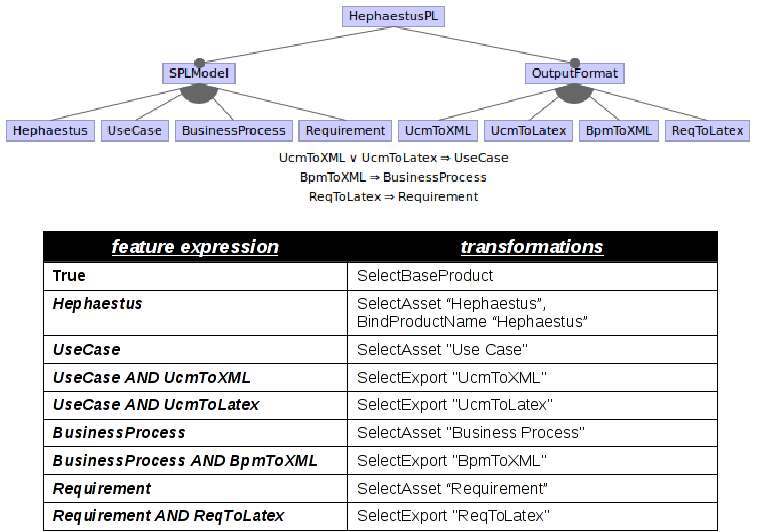
\includegraphics[scale=0.6]{imagens/fm-ck-hpl-req.png}
%\end{center}
%\caption{Hephaestus-PL's FM and CK after introducing \textit{Requirement} asset.}
%\label{fig:fm-ck-hpl-req}
%\end{figure*}

\begin{figure*}[bth]
\begin{center}
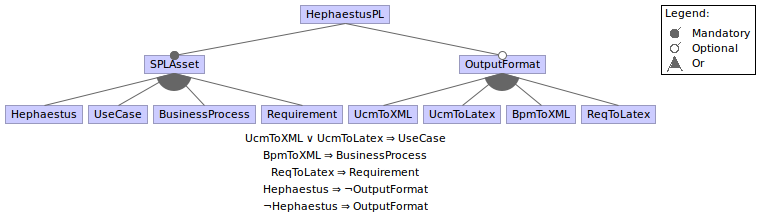
\includegraphics[scale=0.5]{imagens/fm-hpl-ucm-bpm-req.png}
\end{center}
\caption{Hephaestus-PL's FM after introducing \textit{Requirement} asset.}
\label{fig:fm-hpl-ucm-bpm-req}
\end{figure*}

\begin{table}[h]
\begin{center}
\begin{tabular}{||l||l||}
  \hline
  \textbf{Feature Expressions} & \textbf{Transformations}   \\  \hline
  True                         & SelectBaseProduct \\  \hline
  Hephaestus                   & BindProductName "Hephaestus" \\ 
                               & SelectAsset "Hephaestus"   \\
                               & RemoveProductMainFunction \\ \hline
  NOT Hephaestus               & SelectCKParser \\ \hline  
  UseCase                      & SelectAsset "Use Case" \\ \hline
  UseCase AND UcmToXML         & SelectExport "UcmToXML"  \\ \hline
  UseCase AND UcmToLatex       & SelectExport "UcmToLatex" \\ \hline
  BusinessProcess              & SelectAsset "Business Process" \\ \hline
  BusinessProcess AND BpmToXML & SelectExport "BpmToXML" \\ \hline
  Requirement                  & SelectAsset "Requirement" \\ \hline
  Requirement AND ReqToLatex   & SelectExport "ReqToLatex" \\ \hline
\end{tabular}
\caption{Hephaestus-PL's CK after introducing \textit{Requirement} asset.}
\label{tab:ck-hpl-ucm-bpm-req}
\end{center}
\end{table}


Finally, the domain engineer generates a product \hpl{} instance by selecting a product configuration only with the new \textit{Requirement} asset integrated into \hpl{}. She validates if the generated instance contains the correct definitions of the \textit{Requirement} asset into points of variability of the \hpl{} base product and reported the new \hpl{} version to application engineer. Suppose that the validation of the integration of \textit{Requirement} asset into \hpl{} has not been successfully, then it is necessary to return to the assessment of impact in the \hpl{} Kernel's APIs until the validation correct of \hpl{} instance.
 
%The detailed description of the activities of the Hephaestus-PL's reactive process are presented in Appendix B. 

%\subsection{Design Rules for a minimum asset metadata structure}
%\label{sec:designRules}

%\textit{Design Rules} represent a mechanism that would allow reduction of the size of the asset metadata structures in \hpl. Using a inference process into the asset modules, especially the modules that define the data types and the transformations of the asset, it would be possible to get the informations, currently contained in the asset metadata structures, to extend the points of variability of a \hpl{} base product. In this case, we could reduce the size of the asset metadata structures to zero.
%Another intermediate solution that would bring a good reduction of the asset metadata structures would work with two informations, a \textit{acronym} and a \textit{name} of asset, and deriving most of the other informations to the points of variation of \hpl{} with these two variables.

%A atual definicao para a estrutura de meta dados do asset contem 16 fields e esta apresentada na Figure~\ref{fig:metaDataCurrent}. Se analisarmos o preenchimento dessa estrutura para cada um dos assets suportados por Hephaestus-PL, observamos que varios fields dessa estrutura apresentam determinada padronizacao e convencoes no seu preenchimento. Como exemplo, podemos citar o nome do tipo de dados que define as transformacoes dos assets UCM, BPM, Requisitos e Componentes: UseCaseTransformation, BusinessProcessTransformation, RequirementTransformation e ComponentTransformation. Ou seja, todos terminam com a string "Transformation" e comecam com o nome do asset. Poderiamos definir que o nome do tipo de dados algebrico que representa as transformacoes do asset deve ser identificado por \texttt{<assetName>++"Transformation"}. Assim sendo, propomos um conjunto de design rules para o desenvolvimento dos artefatos do asset (tipos abstratos de dados, transformacoes e parser) para minimizar o tamanho da estrutura de meta dados do asset em Hephaestus-PL, otimizando recursos e possibilitando maior automacao na geracao da instancia de Hephaestus com a derivacao automatica de alguns insumos para as operacoes de metaprogramacao, hoje integralmente definidos na estrutura de meta dados do asset (Figure~\ref{fig:exampleMetaDataCurrent}).


%A proposta para uma es%trutura de meta dados minima do asset contem 8 fields (reducao de 50\% do tamanho atual) e esta apresentada na Figure~\ref{fig:proposalMinimumMetaData}. Nesse caso, definimos as seguintes restricoes para permitir a automacao da geracao dos elementos de variacao do asset usados pelas operacoes de metaprogramacao:
%
%\begin{itemize}
%
%\item Os valores definidos para cada field da estrutura de meta dados deve ser unico para aquele field em todos os assets de Hephaestus-PL. Exemplo: não e permitido que o field \texttt{<assetSigla>} seja definido como "XPTO" para o asset A e para o asset B.
%
%\item Implementar nos artefatos do asset as seguintes leis de formacao para a identificacao dos elementos usados na geracao do modulo instancia de Hephaestus:
%
%\begin{itemize}
%
%\item nome do modulo com os tipos abstratos de dados do asset deve ser "Types"
%\item nome do modulo parser do asset deve ser \texttt{<assetModuleParser>}
%\item modulo parser do asset deve estar localizado abaixo do diretorio \texttt{<assetSigla>/Parsers}
%\item nome da funcao parser do asset dentro do modulo do parser (\texttt{<assetModuleParser>}) deve ser \texttt{"parse"++<assetName>++"File"}
%\item nome do modulo que implementa as transformacoes do asset deve ser \texttt{<assetName>}
%\item nome do tipo de dados algebrico que representa o asset deve ser \texttt{<assetName>++"Model"}
%\item nome da funcao que define um produto vazio do asset deve ser \texttt{"empty"++LowerCase<assetSigla>}
%\item nome do tipo de dados algebrico que representa as transformacoes do asset deve ser \texttt{<assetName>++"Transformation"}
%\item nome da funcao que define as transformacoes do asset deve ser \texttt{"transform"++LowerCase<assetSigla>}
%\item nome do parametro que define o asset PL no arquivo de propriedades da entrada de Hephaestus deve ser \texttt{LowerCase<assetName>++"-model"}
%
%\end{itemize}
%
%\end{itemize}
%
%A Figure~\ref{fig:exampleMetaDataMinimum} apresenta um exemplo da estrutura de meta dados minima para o asset UCM.
%
%As regras e definicoes para a automacao da derivacao das informacoes usadas pelas operacoes de metaprogramcao estão sintetizadas na Figure~\ref{fig:metaDataCurrentDerivation} que apresenta a associacao entre os fields da estrutura de meta dados atual e a definicao dos fields a partir da proposta apresentada na Figure~\ref{fig:proposalMinimumMetaData}.


\begin{figure*}[bth]
\begin{center}
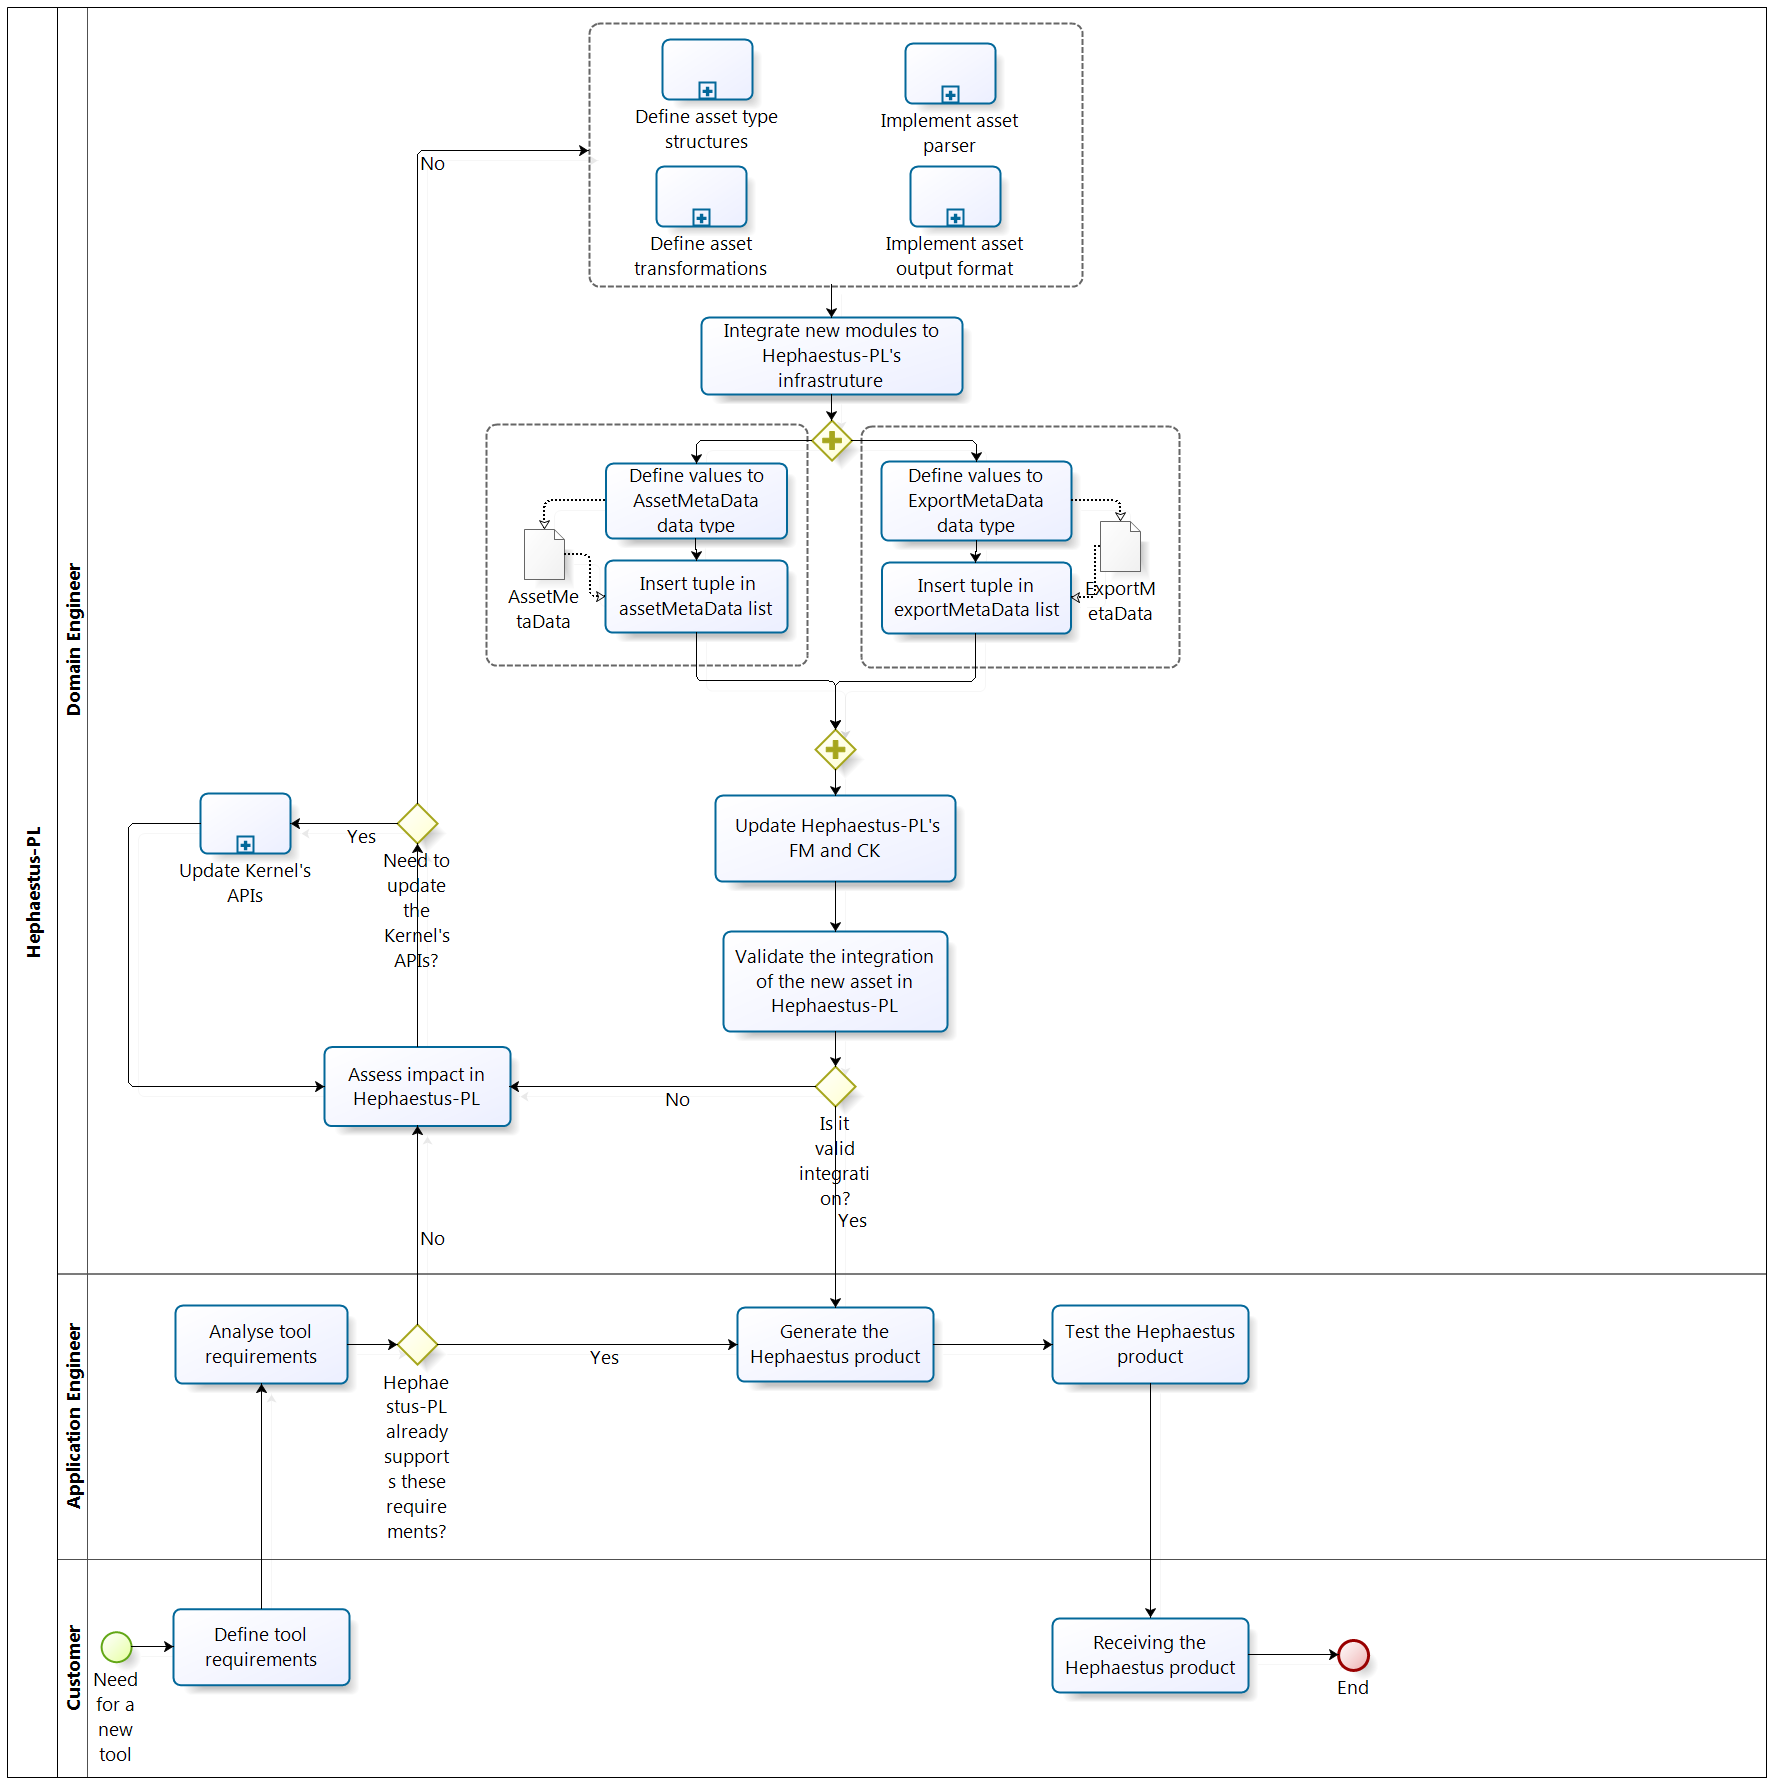
\includegraphics[scale=0.35]{imagens/process.png}
\end{center}
\caption{Reactive Process for introducing new artifacts in \hpl.}
\label{fig:process}
\end{figure*}

%Alem disso, se a variabilidade dos assets nos data types \textit{SPLModel} e \textit{InstanceModel} fosse definida apenas com a adicao de um field que representasse o data type do asset então, poderiamos na geracao de um produto Hephaestus derivar o field e seu tipo a partir dos fields \texttt{<assetSigla>} e \texttt{<assetName>} da estrutura de meta dados minima proposta (ver situacao atual e a proposta na Figure~\ref{fig:proposalAssetSelector}). Atualmente, esse comportamento descrito aqui e observado para os assets UCM, BPM e Requisitos em \hpl. Porem, o asset Componentes não tem esse mesmo comportamento no \textit{SPLModel} e \textit{InstanceModel}, conforme apresentado
%na Section~\ref{sec:implementation}. Assim sendo, precisamos manter os fields  assetSelector' e assetSelector na estrutura de meta dados do asset para atender a extensão desses data types \textit{SPLModel} e \textit{InstanceModel} na geracao da instãncia \hp.
%
%
%
%
%
